
\medskip

%Pour fabriquer un puits dans son jardin, M\up{me} Martin a besoin d'acheter 5 cylindres en
%béton comme celui décrit ci-dessous.
%
%Dans sa remorque, elle a la place pour mettre les 5 cylindres mais elle ne peut
%transporter que $500$~kg au maximum.
%
%À l'aide des caractéristiques du cylindre, déterminer le nombre minimum d'allers-retours
%nécessaires à M\up{me} Martin pour rapporter ses 5 cylindres avec sa remorque.
%
%\begin{tabularx}{\linewidth}{|m{.4\textwidth} X|}\hline
%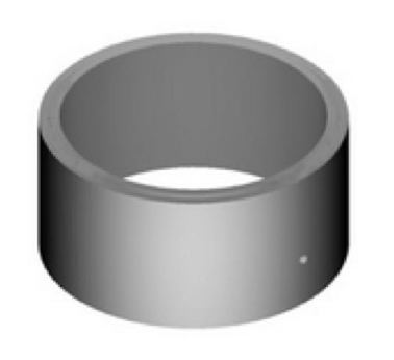
\includegraphics[width=5cm]{cylindre_Asie}&\textbf{Caractéristiques d'un cylindre }:
%
%$\bullet~~$ diamètre intérieur: 90 cm
%
%$\bullet~~$ diamètre extérieur: 101 cm
%
%$\bullet~~$ hauteur: 50 cm
%
%$\bullet~~$ masse volumique du béton: \np{2400} kg/m$^3$\\ \hline
%\multicolumn{2}{|c|}{Rappel: volume d'un cylindre $= \pi  \times  \text{rayon} \times \text{rayon} \times \text{hauteur}$}\\ \hline
%\end{tabularx}
Volume du cylindre extérieur  : $V_1 = \pi \times 50,5^2 \times 50 = \np{127512,5}\pi$~cm$^3$  ; 

Volume du cylindre intérieur  : $V_2 = \pi \times 45^2 \times 50 = \np{101250}\pi$~cm$^3$ ;

Volume béton : $V_1 - V_2 = \np{127512,5}\pi - \np{101250}\pi = \np{26262,5}\pi \approx \np{82506,1}$~cm$^3$ ou environ 82,506~dm$^3$ ou \np{0,0825}~m$^3$.

Un tube a donc une masse égale à : $\np{0,0825} \times \np{2400} = 198$~kg.

Comme $2 \times 198 = 396$ et $3 \times 198 = 554 > 500$, Mme Martin ne peut porter que deux tubes au maximum par voyage  ; elle devra donc porter $2 + 2 + 1 = 5$~tubes. Il lui faudra donc faire trois voyages.

\bigskip

